\chapter{Implementation}

\section{Cineast}

\subsection{Cineast core changes}
UV + texture support in meshes and OBJ loader

\subsection{Model Formats}

The current implementation supports the Wavefront OBJ [\todoMissing{Missing ref}] format as it is comparatively
simple to parse. However, the feature extraction algorithm is agnostic to the original 3D model format and only requires
a 3D mesh consisting of triangles and vertices that contain the following attributes: position and texture coordinates.
Because of Cineast's [\todoMissing{Missing ref}] modular nature it is possible to add parsers for other 3D model formats, or
to extend the currently existing parsers to also read the aforementioned vertex attributes, without having to alter
the feature extraction algorithm.

\subsection{ClusterD2+Color feature extraction}
%What, why (color support), explain assumptions made that were not covered by the paper


In order to compare two or more 3D models for similarity the algorithm must first identify or
extract information that is relevant for the calculation of the similarity metric.
A common way to do so is to reduce the 3D model into an N-dimensional real-valued feature vector which
contains only the most relevant information for a similarity comparison. This feature vector can
then be used to compute a similarity metric, e.g. by calculating the L2 distance between feature vectors.

Since our application allows the user to color their sculptures it makes sense that similarity queries also
take color into account. Hence part of the color information must be contained in the feature vector.
The ClusterD2+Color algorithm described by [\todoMissing{Missing ref}], which was used for this application,
achieves this by creating random sample points on the 3D model's surface according to certain criteria and then
use those sample points to compute a feature vector.

\subsubsection{Sample generation}

Many isosurface extraction algorithms [\todoMissing{Explain this before}], such as the non-adaptive CMS [\todoMissing{Introduce abbr before}]
implementation used in this application, can produce highly tessellated meshes. Opposite to that meshes exported by
3D modeling software are often optimized to have large triangles where the surface has little detail, and small triangles where
the surface is more detailed. Hence it is important that the sample point generation is mostly independent of the triangle sizes
of the mesh, so that meshes of varying levels of tessellation can be compared for similarity effectively.
The ClusterD2+Color algorithm achieves this by making the sampling directly proportional to the surface area of the triangles.
Before any sample points are generated the model is first scaled such that its total surface area equals 100. After that the sample points are generated: a sample point
has a higher chance to be positioned on a large triangle, and a smaller chance to be positioned on a small triangle.
After generating a certain number samples the result is a collection of samples that are uniformly distributed on the mesh's surface. The number of samples
is determined by a function of the integral of the absolute Gaussian curvature over the model's surface.

\subsubsection{Sample Selection}

Once the initial samples have been generated they are filtered and tested for certain criteria.
These criteria differ between shape and color samples.

\subparagraph{Shape Samples}
These samples should convey relevant information about the geometric shape. Previous work done by [\todoMissing{Missing ref; Lee,C.H.,Varshney,A.,Jacobs,D.:Meshsaliency.In:ACMSIGGRAPH’05, pp. 659–666 (2005)}] has
shown that mean curvature is a good indication for visual saliency. The mean curvature of the mesh vertices is computed using Taubin's method [\todoMissing{Missing ref}].
The ClusterD2+Color algorithm computes the mean curvature of each vertex and stores it as a vertex attribute. This mean curvature attribute is then smoothed over the mesh's surface
by Laplacian smoothing [\todoMissing{Missing ref}].

[\todoMissing{Complete}]

\subparagraph{Color Samples}

\subsection{Comparing features for similarity}
L2 distance, Jensen-Shannon divergence, $\chi^2$ distance


\subsection{RESTful API}
OpenAPI, swagger codegen

\section{Voxels}

The foundation of the sculpting feature is based on voxels. In the most basic sense a voxel represents a value on a regular grid
in 3D space [\todoMissing{Missing ref; Wikipedia}]. These voxels are very useful to represent volumetric structures, such as sculptures
or terrain, since they fill the 3D space and each voxel represents one volume element.

\begin{wrapfigure}{R}{0.5\textwidth}
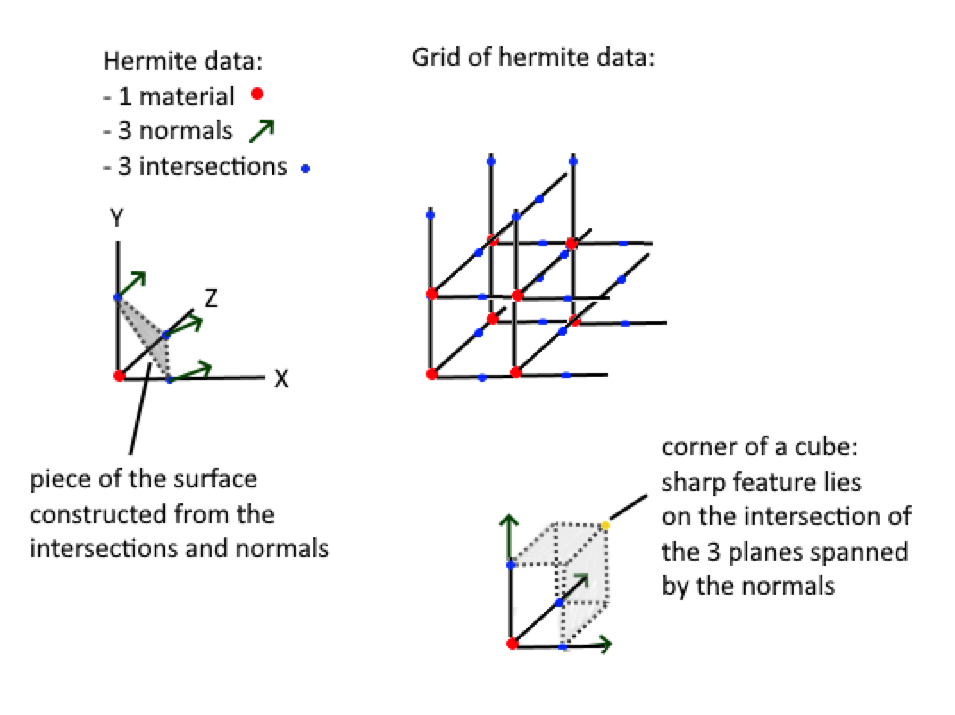
\includegraphics[width=0.5\textwidth]{hermite_data.png}
\caption{Hermite data.}
\label{fig:hermite_data}
\end{wrapfigure}

Since voxels are an abstract representation of volumes they can be visualized in various ways depending on the data the voxel contains.
Usually the data of a voxel consists of a single attribute, a color, in which case the voxel can be visualized e.g. by cubes, spheres, or splats.
More sophisticated voxels contain additional attributes such as normals or texture coordinates. In particular, our application uses voxels that
consist of a 32 bit material ID plus Hermite data [\todoMissing{Missing ref; Dual Contouring}]. Hermite data, first described by [\todoMissing{Missing ref; Dual Contouring}],
consists of two attributes: a material, exact intersection points and normals. Fig. \ref{fig:hermite_data} illustrates the Hermite data and how it can represent
diverse shapes. The Hermite data and voxel material provide enough information to construct the piece of surface represented by a voxel in the form of polygons.

\subsection{Voxel storage}

There are many different data structures to store voxels, the simplest of which is simply storing the voxels' values in large 3D arrays.
Other data structures however need not necessarily store all voxel values on a regular grid. Often there are regions with many voxels of the same value, and
in that case it is beneficial to use a more advanced data structure that can store voxel values more memory efficiently.

The most common method to store voxels in memory is to split the voxels into fixed size blocks or chunks. Within each chunk the voxels are stored in an array. Instead of multi-dimensonal arrays we
use one contiguous linear array to avoid having to dereference multiple pointers for a single access. The index into this linear array can be directly computed from a given X, Y and Z position within the chunk by
the following formula: $index(x, y, z) = x * N * N + y * N + z$, where $N$ is the chunk size.
Our implementation uses a chunk size of 32x32x32. Voxels on the faces towards the positive X, Y and Z axes are padding voxels that always mirror the state of the neighbour voxel in the respective neighbour chunk.
These padding voxels allow the voxel polygonizer to run faster since it entirely removes the need to query neighbour chunks during meshing. This method is described by [\todoMissing{Missing ref; A refined data addressing and processing scheme to accelerate volume raycasting}] in more detail. \\

\todoMissing{Missing ref; Fig in Paper} %See below
\begin{wrapfigure}{R}{0.6\textwidth}
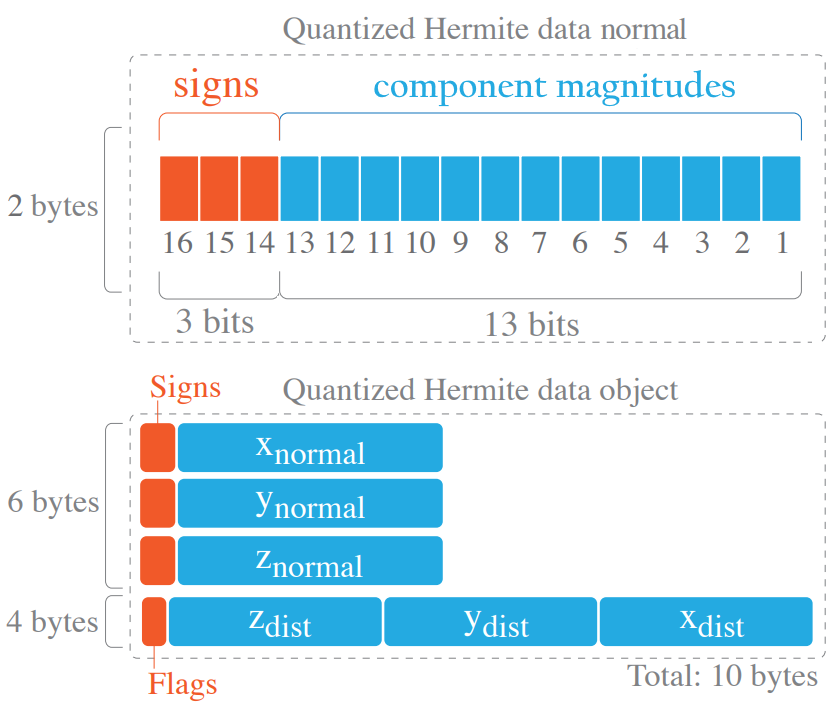
\includegraphics[width=0.4\textwidth]{quantized_hermite_data.png}
\caption{Quantized Hermite data structure. Top: a normal's component magnitudes are packed into 13 bits plus 3 bits for the signs. One normal thus fits into two bytes. Bottom: the entire quantized Hermite data object. $x,y,z_{dist}$ refer to the intersection points. Adapted from [XXX].}
\label{fig:quantized_hermite_data}
\end{wrapfigure}

As previously mentioned the voxels in this application consist of a 32 bit material ID plus Hermite data. Therefore the size of a single voxel in memory is: 4 (material) + $3*3*4$ (three normals, each with three 32 bit float components) + $3*4$ (three intersection points) = 52 bytes in total. Considering that a single chunk contains $32 * 32 * 32 = 32768$ voxels, hence consumes roughly 1.7MB, and one scene can contain many of these chunks,
the main memory will be exhausted rather quickly.
To remedy this issue the Hermite data compression scheme described by [\todoMissing{Missing ref; Fast and Adaptive Polygon Conversion By Means Of Sparse Volumes}] was used.
This quantized Hermite data compression is lossy since it relies on quantizing the floating point values into small integers that are then packed together using bitwise operations. The errors introduced by the compression are
negligible: the exact intersection points remain accurate to a $\frac{1}{1024}$th, respectively less than 0.1\%, of the voxel's edge length. Similarly the maximum error in a normalized normal's component is $\frac{1}{1024}$.
The effective size of the quantized Hermite data is 12 bytes (two of which are struct alignment padding), i.e. only 23\% of the uncompressed size. Fig. \ref{fig:quantized_hermite_data} shows the quantized Hermite data
structure in more detail.\\

\newpage

\begin{wrapfigure}{R}{0.4\textwidth}
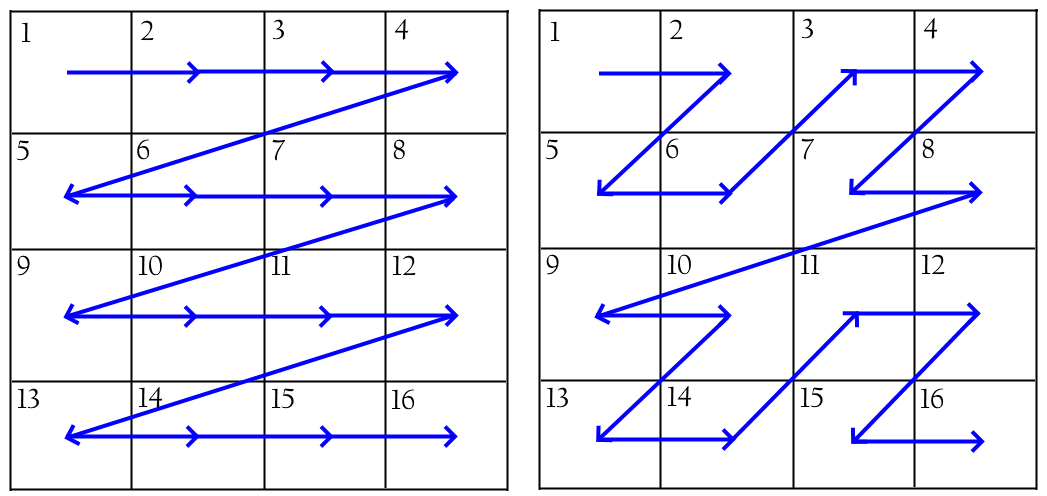
\includegraphics[width=0.4\textwidth]{indexing_order.png}
\caption{Simple linear indexing (left), Z-Order indexing (right). Each square represents a voxel in a 2D array. The blue line represents the order in which they are stored in main memory.}
\label{fig:indexing_order}
\end{wrapfigure}

A further potential optimization is to change the linear array indexing scheme. Modern CPUs have multiple cache layers - each cache layer is a fast memory unit and generally the faster the cache the less
memory it can store. When a program accesses a piece of memory from main memory the CPU loads the surrounding address space into a fixed size cache line, a contiguous piece of the heap memory around the access, into the cache.
If the program then accesses a nearby address again the CPU can read the value from the cache which is a lot faster than reading it from main memory. This is called a cache hit. On the other hand if the program accesses an address further away from the previous access than the size of a cache line the CPU will have to read the value from main memory instead, ergo a cache miss. Hence by optimizing for cache hits a program's speed can be improved if it is memory bound. The most
common access pattern for our voxel storage is to read eight neighbor voxels as a voxel cell for polygonization.
For simplicity's sake we will consider a 2D instead of 3D array: if we use simple linear indexing as shown in Fig. \ref{fig:indexing_order} to read the voxel cell (1, 2, 5, 6) there will be a large address difference between the voxels
on the first and second row. With large arrays this will often lead to cache misses. By instead using Z-Order indexing, also known as Morton indexing, spacially nearby voxels are much more likely to be nearby to each other in the address space, increasing the chance for cache hits. However, such indexing schemes usually have a larger overhead due to the calculation of the index. To compute the Z-Order indices parts of the Libmorton library\footnote{\url{https://github.com/Forceflow/libmorton}} were used and ported to C\#. Unfortunately in our case using Z-Order indexing has made no significant difference, perhaps due to the rather small 32x32x32 chunk size.\todoMissing{Validate this}


\subsection{CMS}

Since the voxels are just an internal volumetric representation some algorithm is required to convert them into something that a computer can
display on the monitor, e.g. a polygonal 3D mesh. From the group of iso-surface and surface contouring algorithms we have decided to use the
Cubical Marching Squares algorithm described by [\todoMissing{Missing ref; CMS}].

\subsubsection{Multi-material extension for CMS}
Algorithm

\subsubsection{Lookup table based implementation}
Lookup table generator, lookup table based algorithm, limitations (time, multi-material support)

\subsection{CSG operations on hermite data}
How union and difference operations work on hermite data, algorithm

\subsection{Rendering}
Vertex colors encode material (RGB, A=texture id), texture array, triplanar texturing shader

\subsection{Voxelizer}
Purpose, explain method used for voxelization (assigning triangles to bins, patching holes, etc.), use of job system

\subsection{SDFs}
Implementation, arbitrary linear transformations by using the inverse to transform space instead of SDF

\section{VR Sculpting}

\subsection{Sculpting features}
General overview of capabilities and functionality, UIs, SteamVR Plugin, etc.

\subsection{Brush properties menu}
Functionalities, color selection (why HSV: you can see most colors at once, as opposed to RGB sliders)

\subsection{Custom brush editing menu}
Explain custom brush tool, why it exists, etc.